\documentclass[11pt,ngerman]{scrartcl}

% standard packages
\usepackage[utf8]{inputenc}  % input in UTF-8
\usepackage[T1]{fontenc}  % output in T1 fonts (westeuropäische Codierung)
\usepackage{lmodern}  % latin modern fonts
\usepackage[ngerman]{babel}  % deutsches Sprachpaket, neue Rechtschreibung

% Seitensetup
\usepackage{scrlayer-scrpage}  % Seitenformatierung durch KOMA-interne Optionen
\usepackage[top=4cm, bottom=4cm]{geometry}  % Seitengeometrie (kann durch KOMA ersetzt werden, hab ich aber nicht geschafft)
\usepackage[hypcap=false]{caption, subcaption}  % caption editing - hypcap warning with hyperref
\usepackage{array}  % table editing

% additional packages
\usepackage{amsmath, amssymb, amstext}  % math packages (American Math Society)
\usepackage{bm}
\usepackage{icomma}  % Kommata in Dezimalzahlen verursachen keinen Abstand mehr
\usepackage{graphicx}  % Bilder einfügen
\usepackage{float} %Bilder placement
\usepackage{pdfpages}  % PDF als vollständige Seiten einfügen
\usepackage{lastpage}  % referenziert die letzte Seite
\usepackage[separate-uncertainty=true]{siunitx}  % bessere Darstellung von Einheiten
\usepackage{makecell} %Dicke Tabellenstriche
\usepackage{longtable}
\usepackage{booktabs}
%\usepackage{datatool}
\usepackage[hidelinks]{hyperref}  % hyperref verlinkt Referenzen - hidelinks entfernt borders um links

% package setups
% Kopf- und Fußzeile durch KOMA
\pagestyle{scrheadings}  % KOMA darf entscheiden
\clearpairofpagestyles  % reset
\setkomafont{pageheadfoot}{\normalfont}  % Standardschrift in Kopf- und Fußzeile
\captionsetup{format=plain, font=small, labelfont=bf} %Better caption, Abbildung ist FETT
%\setlength{\headheight}{27.2pt}  % benötigte Höhe Kopfzeile (warning von scrlayer-scrpage, wird aber automatisch so gerendert, falls diese Option weggelassen wird)
\ihead{Signalleitung}  % Kopf links %Todo Titel ändern
\chead{\textsc{Philipp} Maximilian \\ \textsc{Stark} Matthias}  % Kopf Mitte %Todo Name ändern
\ohead{15 Oktober 2021}  % Kopf rechts %Todo Datum ändern
\cfoot{\pagemark \, / \pageref{LastPage}}  % Fuß Mitte

% Table of Contents
\DeclareTOCStyleEntry{dottedtocline}{section}  % KOMA intern - Inhaltsverzeichnis mit Punkten (nur sections)

%Overbar setup
\newcommand{\overbar}[1]{\mkern 1.5mu\overline{\mkern-1.5mu#1\mkern-1.5mu}\mkern 1.5mu}
% SI
\sisetup{locale = DE}  % deutschsprachige SI-Konvention
\sisetup{quotient-mode = fraction}
\sisetup{per-mode = fraction}
\DeclareSIUnit\px{px}
\DeclareSIUnit\strich{|||}

% citation
\usepackage{csquotes}
\usepackage[backend=biber]{biblatex}
\addbibresource{signalleitung.bib} %Todo .bib befüllen zb.: mit JabRef (Empfehlung der Redaktion)

%Eigene Commands
\newcommand{\der}[2]{\frac{\mathrm{d}#1}{\mathrm{d}#2}}
\newcommand{\pder}[2]{\frac{\partial #1}{\partial #2}}

\begin{document}
\includepdf{Deckblatt_Stark.pdf}
\tableofcontents
\newpage

\section{Aufgabenstellung\label{Auf0}}

\begin{itemize}
	\item Zunächst soll der zeitliche Spannungsverlauf am Anfang und am Ende eines langen
	      Koaxialkabels für verschiedene angelegte Spannungspulse gemessen und erklärt
	      werden.
	\item Dann soll der Reflexionskoeffizient des Kabelendes als Funktion des
	      Abschlusswiederstands bestimmt und so die Kabelimpedanz ermittelt werden.
	\item Weiters soll die Signalgeschwindigkeit im Koaxialkabels bestimmt und so die
	      relative Permittivität des Isolatormaterials des Koaxialkabels bestimmt werden.
	\item Zuletzt sind die Widerstände für einen passiven symmetrischen Verzweiger zu
	      Dimensionieren und die Funktion der Schaltung experimentell zu demonstrieren.
	\item Als Zusatz wird der erste Punkt für eine Sinusspannung auf einen
	      Frequenzbereich von 0.5 bis \SI{6}{MHz} wiederholt.
\end{itemize}

\section{Grundlagen}

% \begin{equation}

% 	\label{eq:Ansatz}
% \end{equation}


Wenn Wechselstrom durch ein Kabel fließt entsteht ein Hertz´scher Dipol, was
große Energieverluste mit sich bringt. Besser eignen sich hier Doppelleitungen,
die dies aufgrund eines Phasenversatzes von $\pi$ und destruktiver Interferenz
ausgleichen. Eine noch bessere Alternative bieten Koaxialkabel. Diese können
als zylindrische Wellenleiter mit kreisförmigen Querschnitt aufgefasst werden.
Wie in der Skizze in \autoref{fig:kabel} ersichtlich, besteht ein Koaxialkabel
aus einem dünnen Innenleiter mit Radius $a$ und einem Koaxialen Außenleiter mit
Radius $b$. \cite{Demtroeder2013}

\begin{center}
	\begin{minipage}[t]{0.5\textwidth}
		\includegraphics[width=\textwidth]{kabel}
		\captionof{figure}{Skizze des Aufbaus eines Koaxialkabels \cite{Demtroeder2013}}
		\label{fig:kabel}
	\end{minipage}
\end{center}



\noindent Ein Leiter kann durch den Leitungswellenwiderstand und den Leitungsbelägen
charakterisiert werden. Die Leitungsbeläge beschreiben folgende Eigenschaften
des Kabels auf die Kabellänge bezogen:

\begin{itemize}
	\item Kapazität
	\item Induktivität
	\item Widerstandsbelag
	\item Querleitwert
\end{itemize}


\noindent Der Kapazitätsbelag $[C']_{\text{SI}} = \si{\farad\per\meter}$ beschreibt die
Kapazität des Leiter pro Länge des Leiter und hängt von der Permittivität
$\varepsilon$ und der Geometrie der Leiteranordung ab.

\noindent Der Induktivitätsbelag $[L']_{\text{SI}} = \si{\henry\per\meter}$ beschreibt
die Induktivität des Leiter pro Länge des Leiter und hängt von der
Permeabilität $\mu$ und auch von der Geometrie der Leiteranordung ab.

\noindent Der Widerstandsbelag ist der Widerstand entlang der Leiterrichtung und dessen
hier relevante zur Länge relative Größe ist der Widerstandsbelag $[R']_{\text{SI}} =
	\si{\ohm\per\meter}$.

\noindent Der Querleitwert ist der Leitwert quer zur Leiterrichtung und beschreibt
wie viel Verlust durch unvollständige Isolierung zustande kommen. Dessen
hier relevante zur Länge relative Größe ist der Ableitungsbelag $[G']_{\text{SI}} =
	\si{\siemens\per\meter}$


\noindent Jede dieser Größen ist vom Material und der Geometrie des Leiter abhängig.

\noindent Unter Verwendung des Induktionsgesetzes erhält man folgende
\autoref{eq:Ansatzwellengleichung}

\begin{align}
	\lim_{\Delta z \to 0} \frac{U(z+\Delta z) - U(z)}{\Delta z} = - L' \der{I}{t}
	\pder{U}{z} = - L' \pder{I}{t}
	\label{eq:Ansatzwellengleichung}
\end{align}

\noindent Betrachtet man einen infinitesimalen kleinen Leitungsabschnitt kann folgendes
Ersatzschaltbild, siehe \autoref{fig:ersatzschaltbild},verwendet werden um die Situation genauer zu erläutern

\begin{figure}
	\begin{center}
		\includegraphics[width=0.7\textwidth]{./figures/ersatzschaltbild.svg.png}
	\end{center}
	\caption{Ersatzschaltbild für infinitesimalen kleinen Leiterabschnitt \cite{wellenleitungskizze}}
	\label{fig:ersatzschaltbild}
\end{figure}

\vspace{2mm}

\noindent Wenn ein harmonisches Wechselspannungssignal auf das Ende einer Signalleitung trifft, wird dieses Signal, je nach Kabel- und Abschlussimpedanz, teilweise reflektiert und in die Abschlussimpedanz übertragen.

\noindent Nun wird folgende Definition des Reflexionskoeffizienten $\rho$
getätigt und die Bedingungen aus den Kirchhoff´schen Regeln aufgestellt. Dabei
beschreiben $U_{r}$ die Amplitude der reflektierte Spannung, $U_e$ die der
einfallenden Spannung und $U_t$ die der transmittierten Spannung. Für  die
Stromstärke gilt dieselbe Notation mit I.

\begin{align}
	\rho & = \frac{U_r}{U_e} \label{eq:rho_durch_u} \\
	U_t  & = U_e + U_r                              \\
	I_t  & = I_e - I_r
\end{align}

\noindent Daraus ergibt sich für die Impedanz des Kabels $Z_K$ und des Anschlusses $Z_A$ folgender Zusammenhang:

\begin{align}
	Z_K = \frac{U_e}{I_e}= \frac{U_r}{I_r} \quad Z_A = \frac{U_t}{I_t}
\end{align}

\noindent Dies ergibt insgesamt für den Reflexionskoeffizienten $\rho$: \cite{Demtroeder2013}

\begin{align}
	\rho = \frac{Z_A - Z_K}{Z_A + Z_K} \label{eq:rho_durch_z}
\end{align}

\noindent Die Ausbreitungsgeschwindigkeit elektromagentische Wellen in Materie
kann wie folgt berechnet werden, siehe \cite{gerthsen}:
\begin{equation}
	v = \frac{c}{\sqrt{\varepsilon_r \mu_r}}
	\label{eq:c_in_m}
\end{equation}

Wobei $c$ die Lichtgeschwindigkeit im Vakuum ist, $\varepsilon_r$ die relative
Permittivität und $\mu_r$ die Permeabilität des Mediums sind.

\newpage

\section{Versuchsanordnung}\label{sec:Versuchsanordnung}

Im Rahmen dieses Versuchs wurden verschiedene Schaltungen dimensioniert. Eine jeweilige Skizze des Schaltplans und eine kurze Erklärung finden sich, der besseren Übersicht halber, immer am Anfang des entsprechenden Versuchs im \autoref{sec:Versuchsdurchführung}.

\vspace{2mm}

\noindent Um die Signale für die entsprechenden Schaltpläne zu erzeugen und auszuwerten wurden folgende Geräte verwendet.

\vspace{2mm}

\noindent Es handelt sich dabei um einen Funktionsgenerator, in \autoref{fig:funki} und ein Oszilloskop, siehe \autoref{fig:oszi}

\vspace{2mm}

\begin{minipage}{\textwidth}
	\begin{minipage}[t]{0.5\textwidth}
		\centering
		\includegraphics[width=\textwidth]{funki}
		\captionbelowof{figure}{Verwendeter Funktionsgenerator}
		\label{fig:funki}
	\end{minipage}
	\vspace{2mm}
	\begin{minipage}[t]{0.50\textwidth}
		\centering
		\includegraphics[width=\textwidth]{oszi}
		\captionof{figure}{Verwendetes Oszilloskop}
		\label{fig:oszi}
	\end{minipage}
	\vspace{1em}
\end{minipage}

\noindent Um die Schaltungen aufzubauen wurden 3 verschiedene Längen von
Koaxialkabeln verwendet, siehe \autoref{fig:kabele}. Um diese zu verbinden
wurden die T-Stücke (3) und Verbindungen (4) aus folgender \autoref{fig:klein}
verwendet. Bei (1) handelt es sich um einen BNC Serienwiderstand, bei (2) um
einen BNC Parallelwiderstand und bei (5) um zwei Abschlusswiederstände mit
jeweils 50 $\Omega$

\vspace{2mm}

\begin{minipage}{\textwidth}
	\begin{minipage}[t]{0.5\textwidth}
		\centering
		\includegraphics[width=\textwidth]{material}
		\captionbelowof{figure}{Verwendete Kabel}
		\label{fig:kabele}
	\end{minipage}
	\vspace{2mm}
	\begin{minipage}[t]{0.50\textwidth}
		\centering
		\includegraphics[angle = 90,width=\textwidth]{kleines}
		\captionof{figure}{Verwendete Stecker und BNC Widerstände}
		\label{fig:klein}
	\end{minipage}
	\vspace{1em}
\end{minipage}

\noindent Für den weiteren Versuchsaufbau werden auch normale Widerstände benötigt, die mithilfe des Steckbretts in den Stromkreis eingebunden werden, siehe \autoref{fig:widerst}. Um den genauen Widerstand dieser zu bestimmen, wird ein digitales Multimeter, \autoref{fig:multi}, verwendet.

\begin{minipage}{\textwidth}
	\begin{minipage}[t]{0.49\textwidth}
		\centering
		\includegraphics[angle =180,width=\textwidth]{widerst}
		\captionbelowof{figure}{Verwendete Widerstände im Steckbrett}
		\label{fig:widerst}
	\end{minipage}
	\vspace{2mm}
	\begin{minipage}[t]{0.49\textwidth}
		\centering
		\includegraphics[width=\textwidth]{multi}
		\captionof{figure}{Verwendetes Multimeter}
		\label{fig:multi}
	\end{minipage}
	\vspace{1em}
\end{minipage}

\newpage

\section{Geräteliste}

\noindent Für die Messungen wurden folgende Geräte verwendet:

\begin{table}[H]
	\captionof{table}{Verwendete Geräte \\ $\Delta \dots$ entsprechende Unsicherheit \\ $L \dots$ Länge der Kabel }
	\begin{center}
		\begin{tabular}{|c|c|c|c|c|} \hline
			\textbf{Gerät}             & \textbf{Typ}      & \textbf{L}    & \textbf{Hersteller}  & $\Delta$              \\ \hline

			Oszilloskop                & DSO-X 2022A       &               & Agilent Technologies &                       \\ \hline
			Funktionsgenerator         & 4063B             &               & BK Precision         &                       \\ \hline
			Multimeter                 & 401456            &               & TTi Aim              &                       \\ \hline
			Koaxialkabel               & RG58 C/U Mil-C-17 & \SI{26.7}{\m} &                      & \SI{0.1}{\m}          \\ \hline
			3 Koaxialkabel             & RG58 C/U Mil-C-17 & \SI{0.53}{\m} &                      & \SI{0.01}{\m}         \\ \hline
			Koaxialkabel               & RG58 C/U Mil-C-17 & \SI{0.27}{\m} &                      & \SI{0.01}{\m}         \\ \hline
			BNC Serienwiderstand       &                   &               &                      &                       \\ \hline
			BNC Parallelwiderstand     &                   &               &                      &                       \\ \hline
			2 BNC T-Stücke             &                   &               &                      &                       \\ \hline
			2 BNC Abschlusswiderstände &                   &               &                      &                       \\ \hline
			Wiederstände               &                   &               &                      &                       \\ \hline
			Steckbrett                 & SYB - 46          &               &                      &                       \\ \hline
			Maßband                    & UKO2 2628         &               & Power-TAPE           & \SI{0.005}{\m\per\m } \\ \hline
		\end{tabular}
	\end{center}
	\label{tab:material}
\end{table}


%*


\section{Versuchsdurchführung \& Messergebnisse}\label{sec:Versuchsdurchführung}

Zunächst wird die Länge der kürzeren Koaxialkabel ermittelt, indem diese
mithilfe des Maßbands vermessen werden. Die dadurch erhaltenen Ergebnisse sind,
der besseren Übersicht halber, bereits in obiger \autoref{tab:material}
hinzugefügt. Die Unsicherheit der Kabel wurde dabei deutlich höher gewählt als
die des Maßbands, aufgrund der Ableseunsicherheit. Die Länge des langen Kabels
war, inklusive der entsprechenden Unsicherheit, gegeben.

\vspace{2mm}

\noindent Für den gesamten Versuchsaufbau wird das Oszilloskop so in den
Schaltkreis geschlossen, dass Channel 1 dem Signaleingang, gelbe Kurve, und
Channel 2 dem Signalausgang, grüne Kurve entspricht.  Weiters wurden die
``Volts per Division`` auf 1:1 gestellt. Und die ``Time per Division`` immer
anhand des jeweiligen Versuchs angepasst. Die jeweiligen Einstellungen können
den entsprechenden Bildern entnommen werden.

\newpage

\subsection{zeitlicher Spannungsverlauf am Anfang und Ende eines Koaxialkabels}

\subsubsection{Variation der Pulsdauer}

Zunächst wird der Stromkreis nach folgenden Schaltplan in \autoref{fig:1a} aufgebaut.

\begin{center}
	\begin{minipage}[t]{0.8\textwidth}
		\includegraphics[width=\textwidth]{1a}
		\captionof{figure}{Skizze des Schaltplans, der für die erste Aufgabe benötigt wird \cite{signalvorlage}}
		\label{fig:1a}
	\end{minipage}
\end{center}

\noindent Der tatsächliche Aufbau ist in folgender \autoref{fig:aufbau} sichtbar.

\begin{center}
	\begin{minipage}[t]{0.7\textwidth}
		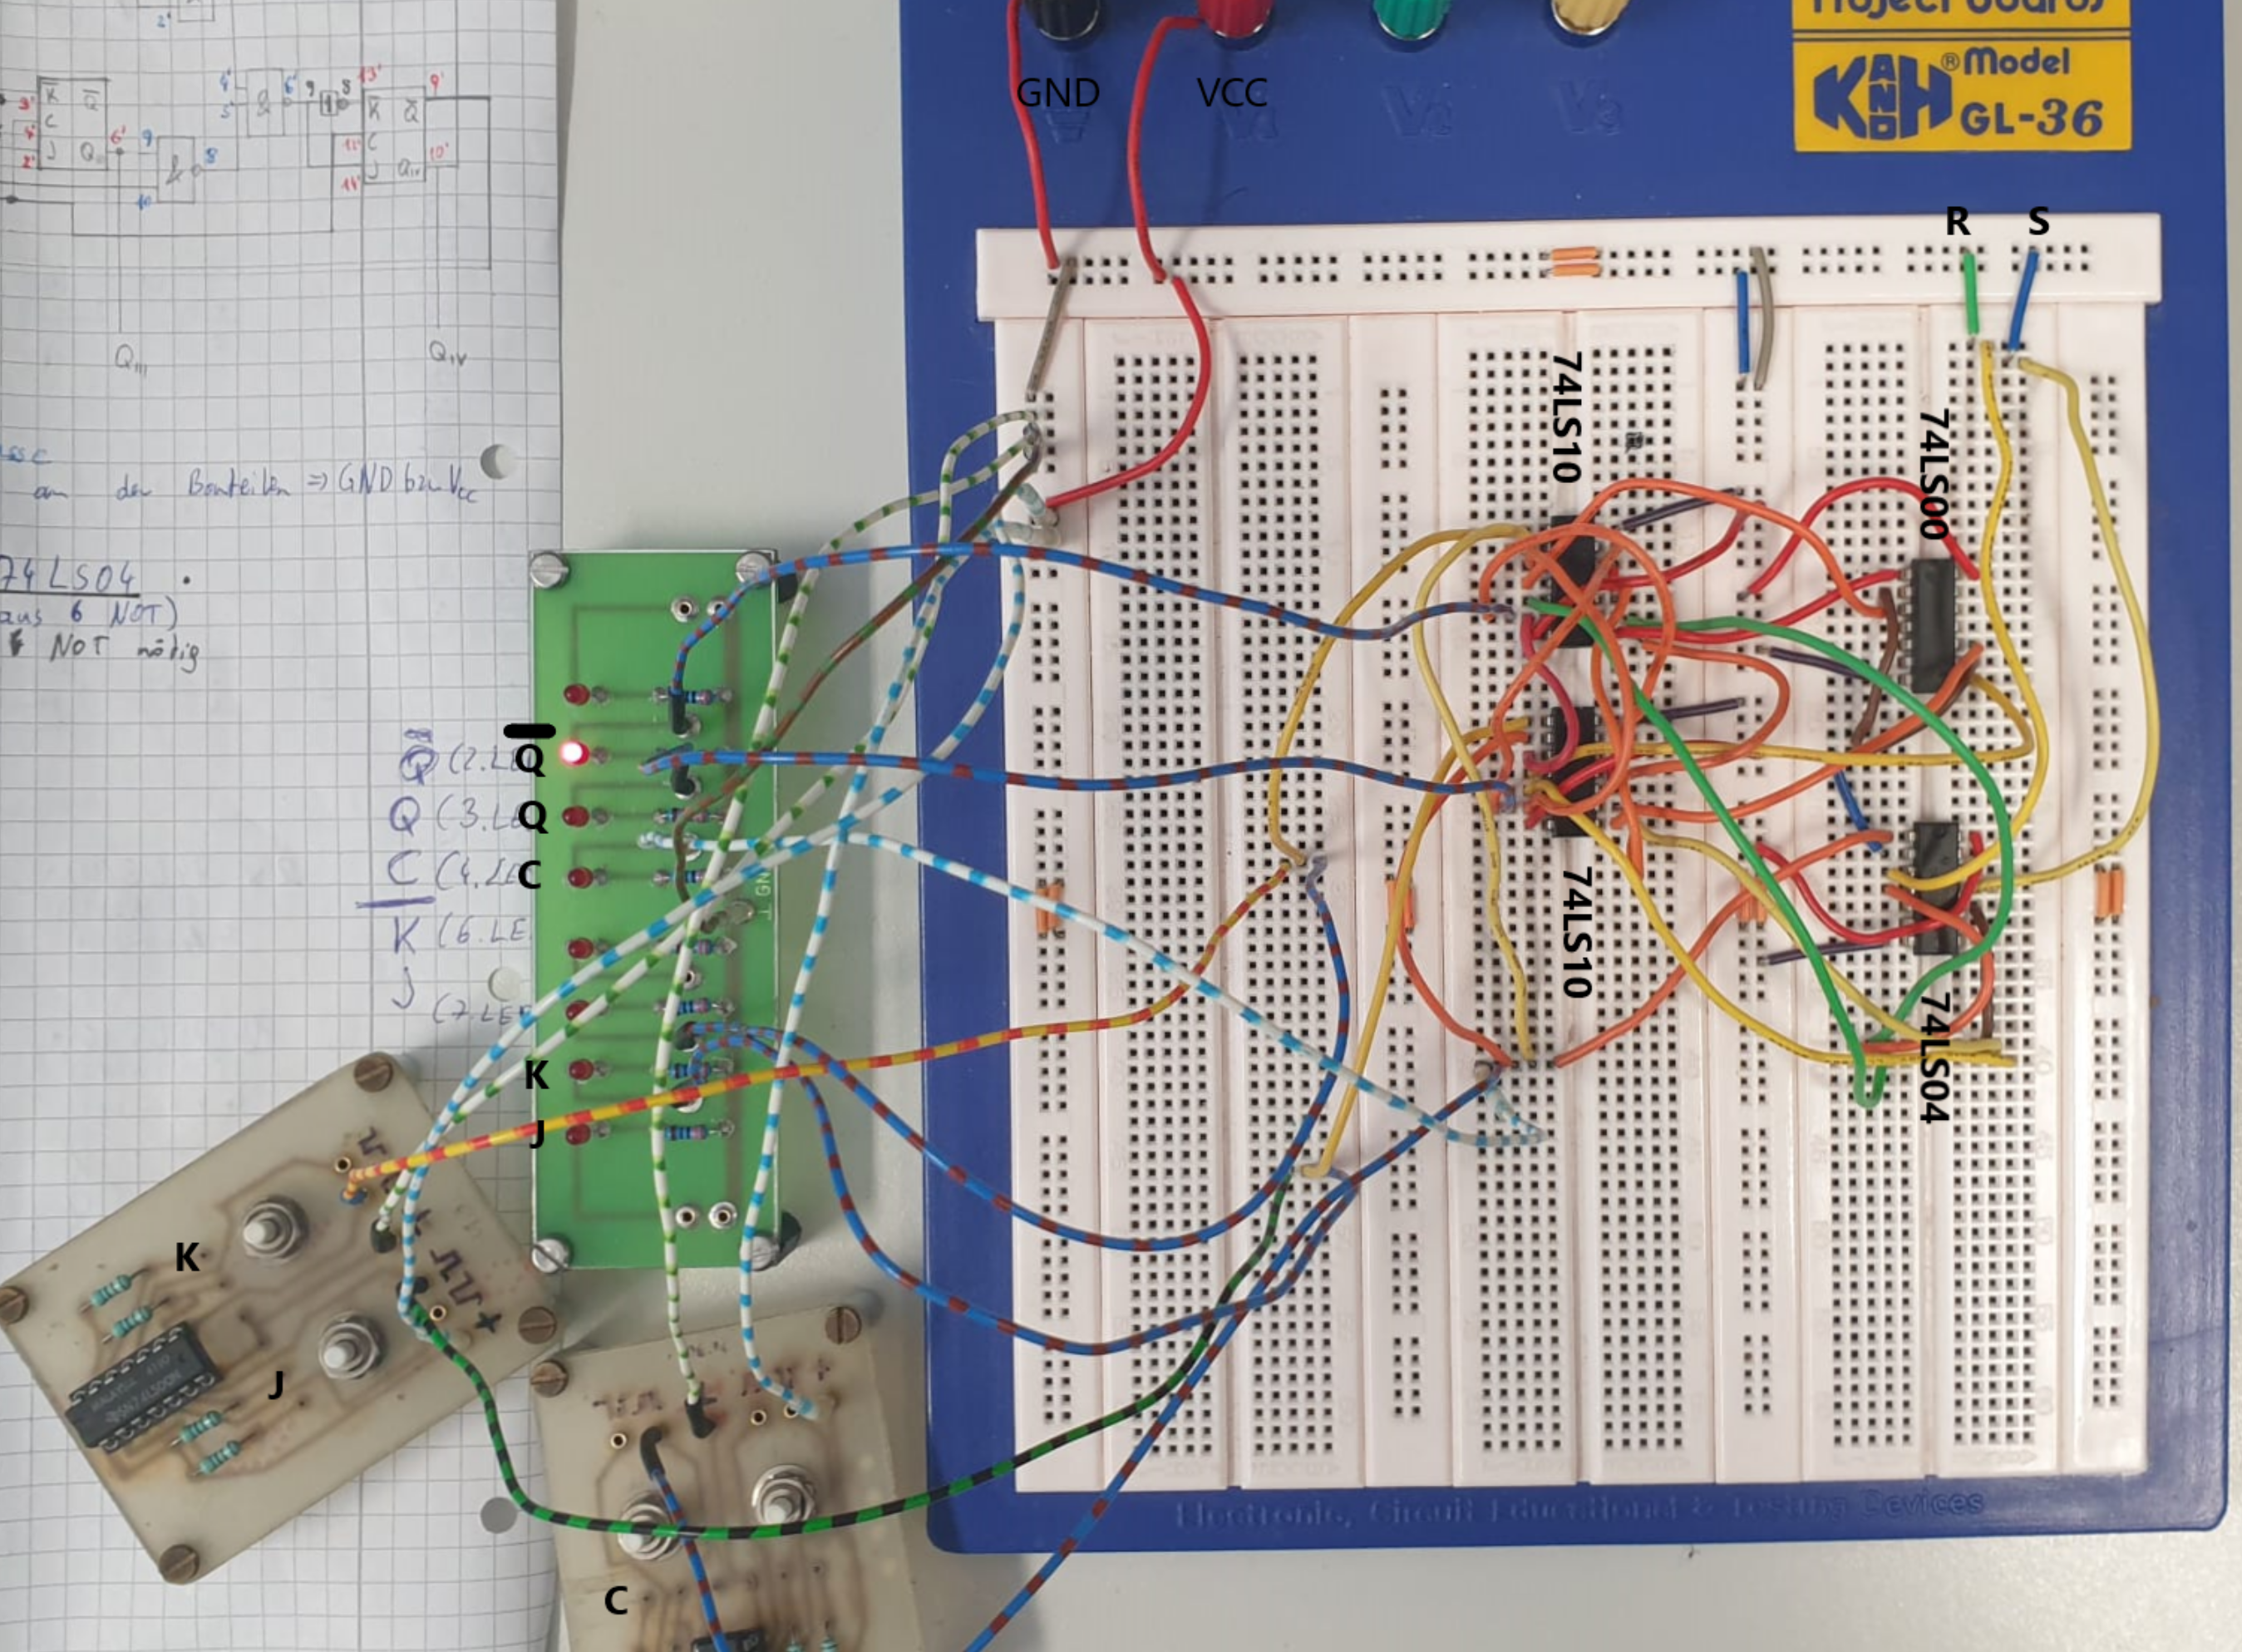
\includegraphics[width=\textwidth]{aufbau}
		\captionof{figure}{Versuchsaufbau für die Messung des Spannungsverlaufs}
		\label{fig:aufbau}
	\end{minipage}
\end{center}

\noindent Zunächst wird mithilfe des Frequenzgenerators ein \SI{300}{\kHz} Signal erzeugt, was mit der Einstellung ``Pulse`` erreicht wird. Die Pulsdauer wird mithilfe der Funktion ``Duty`` auf 3 \% gestellt, was einer Pulsdauer von \SI{100}{\ns} entspricht. Das vom Oszilloskop aufgezeichnete Bild ist in folgender \autoref{fig:3p} ersichtlich.

\begin{center}
	\begin{minipage}[t]{0.7\textwidth}
		\includegraphics[width=\textwidth]{oszi/scope_0_3}
		\captionof{figure}{Vom Oszilloskop aufgezeichnetes Signal bei einem \SI{300}{kHz} Signal und einer Pulsdauer von \SI{100}{ns}}
		\label{fig:3p}
	\end{minipage}
\end{center}

\noindent Nun werden die Cursor ausgerichtet, um das Ablesen der entsprechenden Werte zu ermöglichen, wie in \autoref{fig:3pc} ersichtlich.

\begin{center}
	\begin{minipage}[t]{0.7\textwidth}
		\includegraphics[width=\textwidth]{oszi/scope_0_4}
		\captionof{figure}{Vom Oszilloskop aufgezeichnetes Signal bei einem \SI{300}{kHz} Signal und einer Pulsdauer von \SI{100}{ns} mit eingestelltem Cursor}
		\label{fig:3pc}
	\end{minipage}
\end{center}

\noindent Um besser mit den aufgezeichneten Daten arbeiten zu können, werden diese als ``CSV-Datei`` exportiert und so, gleich wie die ersichtlichen Bilder, direkt vom Oszilloskop auf einen USB-Stick gespeichert.

\noindent Nun werden die Pulsdauer, in Form der ``Duty`` variiert und und die entsprechenden Spannungsverläufe in folgenden Abbildungen aufgelistet.

\begin{minipage}{\textwidth}
	\begin{minipage}[t]{0.5\textwidth}
		\centering
		\includegraphics[width=\textwidth]{oszi/scope_0_8}
		\captionbelowof{figure}{\,Vom \,Oszilloskop \,aufge-\\ zeichnetes Signal bei einem \SI{300}{kHz} Signal\\ und einer ``Duty`` von 0.48 \%}
		\label{fig:0_48p}
	\end{minipage}
	\vspace{2mm}
	\begin{minipage}[t]{0.50\textwidth}
		\centering
		\includegraphics[width=\textwidth]{oszi/scope_0_5}
		\captionof{figure}{\,Vom \,Oszilloskop \,aufge-\\ zeichnetes Signal bei einem \SI{300}{kHz} Signal\\ und einer ``Duty`` von 1 \%}
		\label{fig:1p}
	\end{minipage}
	\vspace{1em}
\end{minipage}

\begin{minipage}{\textwidth}
	\begin{minipage}[t]{0.5\textwidth}
		\centering
		\includegraphics[width=\textwidth]{oszi/scope_0_9}
		\captionbelowof{figure}{\,Vom \,Oszilloskop \,aufge-\\ zeichnetes Signal bei einem \SI{300}{kHz} Signal\\ und einer ``Duty`` von 4 \%}
		\label{fig:4p}
	\end{minipage}
	\vspace{2mm}
	\begin{minipage}[t]{0.50\textwidth}
		\centering
		\includegraphics[width=\textwidth]{oszi/scope_0_12}
		\captionof{figure}{\,Vom \,Oszilloskop \,aufge-\\ zeichnetes Signal bei einem \SI{300}{kHz} Signal\\ und einer ``Duty`` von 8 \%}
		\label{fig:8p}
	\end{minipage}
	\vspace{1em}
\end{minipage}

\begin{minipage}{\textwidth}
	\begin{minipage}[t]{0.5\textwidth}
		\centering
		\includegraphics[width=\textwidth]{oszi/scope_0_13}
		\captionbelowof{figure}{\,Vom \,Oszilloskop \,aufge-\\ zeichnetes Signal bei einem \SI{300}{kHz} Signal\\ und einer ``Duty`` von 9 \%}
		\label{fig:9p}
	\end{minipage}
	\vspace{2mm}
	\begin{minipage}[t]{0.50\textwidth}
		\centering
		\includegraphics[width=\textwidth]{oszi/scope_0_16}
		\captionof{figure}{\,Vom \,Oszilloskop \,aufge-\\ zeichnetes Signal bei einem \SI{300}{kHz} Signal\\ und einer ``Duty`` von 20 \%}
		\label{fig:20p}
	\end{minipage}
	\vspace{1em}
\end{minipage}

\begin{minipage}{\textwidth}
	\begin{minipage}[t]{0.5\textwidth}
		\centering
		\includegraphics[width=\textwidth]{oszi/scope_0_17}
		\captionbelowof{figure}{\,Vom \,Oszilloskop \,aufge-\\ zeichnetes Signal bei einem \SI{300}{kHz} Signal\\ und einer ``Duty`` von 30 \%}
		\label{fig:30p}
	\end{minipage}
	\vspace{2mm}
	\begin{minipage}[t]{0.50\textwidth}
		\centering
		\includegraphics[width=\textwidth]{oszi/scope_0_20}
		\captionof{figure}{\,Vom \,Oszilloskop \,aufge-\\ zeichnetes Signal bei einem \SI{300}{kHz} Signal\\ und einer ``Duty`` von 40 \%}
		\label{fig:40p}
	\end{minipage}
	\vspace{1em}
\end{minipage}

\subsubsection{Erhöhung des Innenwiderstands durch Serienwiderstand}

Nun wird der Stromkreis nach folgender Skizze in \autoref{fig:1b} des Schaltplans aufgebaut.

\begin{center}
	\begin{minipage}[t]{0.8\textwidth}
		\includegraphics[width=\textwidth]{1b}
		\captionof{figure}{Skizze des Schaltplans mit Serienwiderstand \cite{signalvorlage}}
		\label{fig:1b}
	\end{minipage}
\end{center}

\noindent Dazu wird der BNC-Serienwiederstand aus \autoref{fig:klein} verwendet.

\noindent Mithilfe des Frequenzgenerators wird wieder ein \SI{300}{kHz} Signal erzeugt. Für die Pulsdauer wird ein Signal von 1 $\mu$s verwendet, was einer ``Duty`` von 30 \% entspricht.

\vspace{2mm}

\noindent Das so erzeugte Spannungsbild ist in folgender \autoref{fig:1b30p} zu sehen.

\begin{center}
	\begin{minipage}[t]{0.7\textwidth}
		\includegraphics[width=\textwidth]{oszi/scope_0_21}
		\captionof{figure}{Vom Oszilloskop aufgezeichnetes Signal bei einem \SI{300}{kHz} Signal und einer Pulsdauer  1 $\mu$s mit Serienwiderstand}
		\label{fig:1b30p}
	\end{minipage}
\end{center}



\subsubsection{Erhöhung des Innenwiderstands durch Parallelwiderstand}

\noindent Nun wird der Serienwiderstand durch einen Parallelwiederstand getauscht, sodass folgender Schaltplan aus \autoref{fig:1c} entsteht.

\begin{center}
	\begin{minipage}[t]{0.8\textwidth}
		\includegraphics[width=\textwidth]{1c}
		\captionof{figure}{Skizze des Schaltplans mit Parallelwiderstand \cite{signalvorlage}}
		\label{fig:1c}
	\end{minipage}
\end{center}

\noindent Dazu wird der BNC-Parallelwiederstand aus \autoref{fig:klein} verwendet.

\noindent Das aufgezeichnete Signal des Oszilloskops bei einem \SI{300}{kHz} Signal erzeugt und einer Pulsdauer von 1 $\mu$s ist in folgender \autoref{fig:1c30p} ersichtlich.

\begin{center}
	\begin{minipage}[t]{0.7\textwidth}
		\includegraphics[width=\textwidth]{oszi/scope_0_25}
		\captionof{figure}{Vom Oszilloskop aufgezeichnetes Signal bei einem \SI{300}{kHz} Signal und einer Pulsdauer  1 $\mu$s mit Parallelwiderstand}
		\label{fig:1c30p}
	\end{minipage}
\end{center}




\subsection{Reflexionskoeffizient des Kabels und Kabelimpedanz}

Um den Reflexionskoeffizienten des Kabel zu bestimmen, müssen zunächst die
genauen Werte der Widerstände am Steckbrett gemessen werden, da diese nicht mit
dem angeschriebenen Werten der Widerstände übereinstimmen. Dies geschieht mit
dem Multimeter aus \autoref{fig:multi}. Der besseren Übersicht halber, werden
die erhaltenen Werte erst später in \autoref{tab:rho} aufgelistet.

\vspace{2mm}

\noindent Der Schaltplan für den Versuchsaufbau ist in folgender Skizze in \autoref{fig:2b} ersichtlich.

\begin{center}
	\begin{minipage}[t]{0.8\textwidth}
		\includegraphics[width=\textwidth]{2b}
		\captionof{figure}{Skizze des Schaltplans für den Reflexionskoeffizient des Kabels \cite{signalvorlage}}
		\label{fig:2b}
	\end{minipage}
\end{center}

\noindent Der tatsächliche Versuchsaufbau ist in folgender \autoref{fig:aufbau2} ersichtlich.

\begin{center}
	\begin{minipage}[t]{0.7\textwidth}
		\includegraphics[width=\textwidth]{aufbau2}
		\captionof{figure}{Versuchsaufbau für den Reflexionskoeffizient des Kabels}
		\label{fig:aufbau2}
	\end{minipage}
\end{center}

\noindent Dabei ist zu beachten, dass sich im Koaxialkabel sowohl Hin als auch Retourleiter befinden und so die beiden Kabel, die an den Widerstand angeschlossen werden an die gleiche Steckbuchse des Koaxialkabel geführt werden.

\vspace{2mm}

\noindent Um bessere Werte zu erhalten wurde die Mittlung von 64 ``Sample``  am Oszilloskop eingeschaltet.

\vspace{2mm}

\noindent Nun wurde mithilfe der Cursor die Referenzspannung des Signals nach dem ersten ``rising edge`` gemessen und auch der letzte Spannungswert am letzten Peak, in \autoref{fig:wid} mit 1 markiert, gemessen.

\begin{center}
	\begin{minipage}[t]{0.7\textwidth}
		\includegraphics[width=\textwidth]{oszi/scope_0_26}
		\captionof{figure}{Vom Oszilloskop aufgezeichnetes Signal bei \SI{300}{kHz} und einer Pulsdauer  1 $\mu$s für die Messung des Widerstands}
		\label{fig:wid}
	\end{minipage}
\end{center}

\noindent Die so erhaltenen Ergebnisse sind in folgender Tabelle aufgelistet.

\begin{table}[H]
	\captionof{table}{Abgelesene Werte für die Widerstände \\ $R \dots$
		gemessener Widerstand mit dem Multimeter mit entsprechender Unsicherheit \\
		$U_{e} \dots$ gemessene Referenzspannung \\ $U_r \dots$ gemessener Wert für die
		reflektierte Spannung}
	\begin{center}
		\begin{tabular}{|S|c|c|} \hline
			{R / $\Omega$} & { $U_{e}$ / V} & {$U_r$ / V} \\ \hline

			1794(17)       & 1.019          & 0.937       \\
			1195(12)       & 1.019          & 0.903       \\
			677(7)         & 1.031          & 0.841       \\
			330.1(6)       & 1.035          & 0.713       \\
			179.5(3)       & 1.027          & 0.539       \\
			100.1(2)       & 1.032          & 0.306       \\
			68.10(16)      & 1.031          & 0.132       \\
			47.12(13)      & 1.027          & -0.051      \\
			33.02(10)      & 1.015          & -0.202      \\
			12.14(8)       & 1.015          & -0.585      \\
			18.04(10)      & 1.027          & -0.434      \\
			\hline
		\end{tabular}
	\end{center}
	\label{rwerte}
\end{table}


%*
\noindent Nun wird der Reflexionskoeffizient bei Verwendung des BNC
Abschlusswiderstand bestimmt, was in folgender \autoref{fig:nachtrag} sichtbar
ist. Da dieser wie in der \autoref{fig:nachtrag} ersichtlich die Reflexion
auslöscht ist der BNC Abschlusswiderstand gleich groß wie die Kabelimpedanz.

\begin{center}
	\begin{minipage}[t]{0.7\textwidth}
		\includegraphics[width=\textwidth]{oszi/scope_0_30}
		\captionof{figure}{Vom Oszilloskop aufgezeichnetes Signal bei \SI{300}{kHz} bei der Verwendung des BNC Abschlusswiderstands}
		\label{fig:nachtrag}
	\end{minipage}
\end{center}

\subsection{Signalgeschwindigkeit des Kabels und Permitivität des Isolatormaterials}

Um die Signalgeschwindigkeit des Kabels bestimmen zu könne, wird die Zeit
gemessen vom Signalanfang bis zum Retoursignal gemessen und daraus die
Periodendauer $T$, um die doppelte Länge des Kabels zurückzulegen, bestimmt. Um
diese zu bestimmen, wird der Abstand der gelben und grünen Linie in
\autoref{fig:30p} bestimmt.

\vspace{2mm}

\noindent Die gemessene Laufzeit $T$ ist:
\begin{equation}
	T = \SI{272(5)}{\ns}
	\label{eq:laufzeit}
\end{equation}

\noindent Die Kabellänge ist in der Geräteliste spezifiziert, siehe \autoref{tab:material}.

\subsection{Schaltung mit Widerständen}

\noindent Nun wird der Schaltplan nach folgender Skizze aus \autoref{fig:4} aufgebaut.

\begin{center}
	\begin{minipage}[t]{0.8\textwidth}
		\includegraphics[width=\textwidth]{4}
		\captionof{figure}{Skizze des Schaltplans für die Schaltung mit Widerständen \cite{signalvorlage}}
		\label{fig:4}
	\end{minipage}
\end{center}

\noindent Der tatsächliche Versuchsaufbau ist in \autoref{fig:aufbau4} ersichtlich.

\begin{center}
	\begin{minipage}[t]{0.7\textwidth}
		\includegraphics[width=\textwidth]{aufbau4}
		\captionof{figure}{Versuchsaufbau für die Schaltung mit Widerständen}
		\label{fig:aufbau4}
	\end{minipage}
\end{center}




\subsection{Sinusspannung}

\noindent Nun wird der Versuch wieder nach den Schaltplan aus \autoref{fig:1a} aufgebaut und eine Sinusspannung mit einer Frequenz von \SI{0.5}{MHz} angelegt.
\noindent Das so erzeugte Signal des Oszilloskops ist in folgender \autoref{fig:0_5h} sichtbar.

\begin{center}
	\begin{minipage}[t]{0.7\textwidth}
		\includegraphics[width=\textwidth]{oszi/scope_0_36}
		\captionof{figure}{Vom Oszilloskop aufgezeichnetes Signal bei einer Sinusspannung und einem \SI{0.5}{MHz} Signal}
		\label{fig:0_5h}
	\end{minipage}
\end{center}

\noindent Nun wird die Frequenz erhöht und dadurch folgende Signale erzeugt.

\vspace{2mm}

\begin{minipage}{\textwidth}
	\begin{minipage}[t]{0.5\textwidth}
		\centering
		\includegraphics[width=\textwidth]{oszi/scope_0_35}
		\captionbelowof{figure}{\,Vom \,Oszilloskop \,aufge-\\ zeichnetes Signal bei einer Sinusspannung \\ und einem \SI{1}{MHz} Signal}
		\label{fig:1h}
	\end{minipage}
	\vspace{2mm}
	\begin{minipage}[t]{0.50\textwidth}
		\centering
		\includegraphics[width=\textwidth]{oszi/scope_0_39}
		\captionof{figure}{\,Vom \,Oszilloskop \,aufge-\\ zeichnetes Signal bei einer Sinusspannung \\ und einem \SI{2}{MHz} Signal}
		\label{fig:2h}
	\end{minipage}
	\vspace{1em}
\end{minipage}

\begin{minipage}{\textwidth}
	\begin{minipage}[t]{0.5\textwidth}
		\centering
		\includegraphics[width=\textwidth]{oszi/scope_0_40}
		\captionbelowof{figure}{\,Vom \,Oszilloskop \,aufge-\\ zeichnetes Signal bei einer Sinusspannung \\ und einem \SI{3}{MHz} Signal}
		\label{fig:3h}
	\end{minipage}
	\vspace{2mm}
	\begin{minipage}[t]{0.50\textwidth}
		\centering
		\includegraphics[width=\textwidth]{oszi/scope_0_43}
		\captionof{figure}{\,Vom \,Oszilloskop \,aufge-\\ zeichnetes Signal bei einer Sinusspannung \\ und einem \SI{4}{MHz} Signal}
		\label{fig:4h}
	\end{minipage}
	\vspace{1em}
\end{minipage}

\begin{minipage}{\textwidth}
	\begin{minipage}[t]{0.5\textwidth}
		\centering
		\includegraphics[width=\textwidth]{oszi/scope_0_44}
		\captionbelowof{figure}{\,Vom \,Oszilloskop \,aufge-\\ zeichnetes Signal bei einer Sinusspannung \\ und einem \SI{5}{MHz} Signal}
		\label{fig:5h}
	\end{minipage}
	\vspace{2mm}
	\begin{minipage}[t]{0.50\textwidth}
		\centering
		\includegraphics[width=\textwidth]{oszi/scope_0_47}
		\captionof{figure}{\,Vom \,Oszilloskop \,aufge-\\ zeichnetes Signal bei einer Sinusspannung \\ und einem \SI{6}{MHz} Signal}
		\label{fig:6h}
	\end{minipage}
	\vspace{1em}
\end{minipage}






\section{Auswertung}

\noindent Um zu sehen wie sich die Unsicherheit der Messungen bis in die Ergebnisse
fortplanzt, ist \autoref{eq:Unsicherheitsfortpflanzung} verwendet worden.
Die Grundlagen dieser Gleichung stammen von den Powerpointfolien von
GUM.\cite{WolfgangKessel2004} Die Verallgemeinerung ist von Wikipedia entnommen
worden \cite{2020Fehler}.
Für die Auswertung ist die Progammiersprache Python im speziellen das
Packet \verb#scipy#, zur Hilfe genommen worden.

\begin{equation}
	\label{eq:Unsicherheitsfortpflanzung}
	V_y = J(x) \cdot V_x \cdot J^{T}(x)
\end{equation}

\noindent Wobei $V_y$ und $V_x$ die Kovarianzmatrizen von den Vektoren $\bm{y}$ und $\bm{x}$ sind.
$\bm{x}$ ist der Vektor der Eingangsvariablen und $\bm{y}$ ist der Vektor der Ausgangsvariablen.
$J$ ist die Jakobimatrix der vektorwertigen Funktion $\bm{y} = \vec{F}(\bm{x})$.
So lassen sich die Komponenten der Matrix relativ einfach anschreiben $J_{ij}(x) = \frac{\partial{y_i}}{\partial{x_j}}(x)$.
Damit man die Unsicherheit der einzelnen Variablen $y_i$ bekommt, muss nur die Quadratwurzel des i-ten Diagonalelementes der
$\bm{y}$-Kovarianzmatrix genommen werden $u_i= \sqrt{\mathrm{diag}(V_y)_i}$.
Da in diesem Experiment meistens nur skalare Funktionen untersucht werden, vereinfacht
sich die \autoref{eq:Unsicherheitsfortpflanzung} dramatisch und die Unsicherheit
der Variable $y$ lässt sich einfach so berechnen:

\begin{equation}
	\label{eq:graduncentainty}
	u_y = \sqrt{\mathrm{grad} y^T \cdot V_x \cdot \mathrm{grad} y}
\end{equation}


\subsection{zeitlicher Spannungsverlauf am Anfang und Ende eines Koaxialkabels}


\subsubsection{Variation der Pulsdauer}

Zunächst sind die Peaks des ausgesendeten und des reflektierten Signals klar getrennt sichtbar.
Betrachtet man die entsprechenden \autoref{fig:8p} und \autoref{fig:9p} so stellt man fest, dass genau dazwischen ein Zeitpunkt existiert, bei dem das Sendezeit des Anfangs gesendete Signal genau mit der Umlaufzeit übereinstimmt.
Danach  überlagern sich die Spannungen der Signale, was in den darauffolgenden Bildern klar ersichtlich ist.

\subsubsection{Erhöhung des Innenwiderstands durch Serienwiderstand}

Die Erhöhung des Innenwiderstand der Quelle durch Serienschaltung, erlaubt es,
dass das Retoursignal nochmal mit einem Reflexionskoeffizienten, der in
Intervall von $0 \leq \rho \leq 1$ liegt, reflektiert wird. Das Eingangs und
Ausgangssignal überlagern sich mit den Reflexionen. Wenn das Signal aufhört zu
senden beginnt das System sich auszuschwingen, wie in \autoref{fig:1b30p}
ersichtlich.

\subsubsection{Erhöhung des Innenwiderstands durch Parallelwiderstand}

Die Verringerung des Innenwiderstand der Quelle durch Parallelschaltung,
erlaubt es, dass das Retoursignal nochmal mit einem Reflexionskoeffizienten,
der in Intervall von $-1 \leq \rho \leq 0$ liegt, reflektiert wird. Das
Eingangs und Ausgangssignal überlagern sich mit den Reflexionen. Aufgrund des
negativen Vorzeichens, findet Signalinversion statt, wodurch das empfangene
Retoursignal das sendene Signal abschwächt. Bei schwächerer Verzeichnung werden
wieder positive Sprünge sichtbar, bis sich das Signal schließlich im Positiven,
beim Eingangssignal, einpendeln würde. Aufgrund des Ausschalten des Signals,
fällt dieses ins Negative und pendelt sich schließlich um den Nullpunkt ein,
wie in \autoref{fig:1c30p} ersichtlich.

\subsection{Reflexionskoeffizient des Kabels und Kabelimpedanz}

Die reflektierten Spannungen werden durch den entsprechenden Wert der
Referenzspannung dividiert, wodurch Werte für den Reflexionskoeffizienten
ermittelt werden können.

\noindent Dadurch ergeben sich folgende Werte, siehe \autoref{tab:rho}. Die Unsicherheiten sind dabei, wie
bereits zuvor erwähnt, mittels Computer ermittelt worden.

%*tab
\begin{table}[H]
	\caption{Werte für die mit \autoref{eq:rho_durch_u} errechneten Reflexionskoeffizienten $\rho$ }
	\label{tab:rho}
	\begin{center}
		\begin{tabular}{lrr}
	\toprule
	{} & $\rho$ & $\Delta \rho$ \\
	\midrule
	0  & 0.92   & 0.05          \\
	1  & 0.89   & 0.05          \\
	2  & 0.82   & 0.05          \\
	3  & 0.69   & 0.05          \\
	4  & 0.52   & 0.04          \\
	5  & 0.30   & 0.04          \\
	6  & 0.13   & 0.03          \\
	7  & -0.05  & 0.03          \\
	8  & -0.20  & 0.03          \\
	9  & -0.58  & 0.04          \\
	10 & -0.42  & 0.04          \\
	\bottomrule
\end{tabular}

	\end{center}
\end{table}


\noindent Die so erhaltenen Daten werden nun an der theoretischen Kurve, siehe
\autoref{eq:rho_durch_z}, gefittet, wodurch folgender Plot entsteht.

%*plot
\begin{figure}[H]
	\begin{center}
		\includegraphics[width=0.95\textwidth]{./figures/fit_with_data_0.png}
	\end{center}
	\caption{Gemessene Werte für den Reflexionskoeffizienten $\rho$ gegen den
		Anschlusswiderstand $Z_A$ geplottet und an die theoretische Kurve gefittet um
		die unbekannte Kabelimpedanz $Z_K$ zu bestimmen.}
	\label{fig:rhofit}
\end{figure}


\noindent Indem die Kurve durch Non-Linear Fit Methoden gefittet worden ist und $Z_K$
als Fitparameter genommen worden ist folgender Wert,wie in
\autoref{fig:rhofit}, ermittelt worden:

\begin{equation}
	Z_K = \SI{51.6(16)}{\ohm}
\end{equation}

\noindent Eine andere Methode wäre gewesen den Nullpunkt mittels linearen Interpolation
zwischen dem Wert, der gerade ober 0 ist, und dem Wert, der gerade unter 0
ist, zu machen. Da in diesem Punkt gerade der Reflexionskoeffizient 0 ist
gilt folgende \autoref{eq:zknull}:

\begin{equation}
	Z_K = Z_A \quad \mathrm{wobei}\; \rho = 0
	\label{eq:zknull}
\end{equation}

%*ert

\subsection{Signalgeschwindigkeit des Kabels und Permitivität des Isolatormaterials}

\noindent Anhand der gemessenen Umlaufzeit $T$ und der Länge des Kabels $l$ erhält man
dadurch die Geschwindigkeit der Kabels, was folgende Werte liefert.
\begin{equation}
	v_{\text{Signal}} = \frac{2l}{T} = \frac{2 \num{26.7(1)}}{\num{272(5)e-9}} \si{\meter\per\second} = \SI{1.96(5)e8}{\meter\per\second}
	\label{eq:Signalgeschwindigkeit}
\end{equation}

\noindent Verwendet man nun die so gefundene Signalgeschwindingkeit mit der
\autoref{eq:c_in_m} und formt auf $\varepsilon_r$ um, kann die Permitivität des
Isolatormaterial bestimmt werden, da es ein Dielektrikum ist und daher ein
relative Permiabilität von $\mu_r = 1$ hat.

\begin{equation}
	\varepsilon_r = \left( \frac{c}{v_{\text{Signal}}} \right)^2 = \SI{2.33(11)}{\farad\per\meter}
	\label{eq:permittivity}
\end{equation}

\subsection{Schaltung mit Widerständen}

Aufgrund des Aufbaue ist, wie im Diagramm ersichtlich, dass die Widerstände
richtig gewählt worden sind, sodass keine Reflexion möglich ist und dadurch die
Signalintegrität verbessert wird und dadurch maximale Leistungsübertragung
stattfindet. Durch diese Widerstände wird daher der ideale Aufbau für eine
Signalquelle und 2 Empfänger repräsentiert. Bei einer Änderung der Länge des
Kabels oder Widerstände am Kabelende müsste der jeweils andere Parameter
angepasst werden.

\subsection{Sinusspannung}

Der Verlauf der Sinusspannung, kann mit der Mechanik einer stehenden Welle
verglichen werden. Dies ist daran erkennbar, dass mit zunehmender Frequenz die
Amplituden sowohl anwachsen als auch schrumpfen. Dies ist aufgrund von
destruktiver Interferenz erklärbar. Theoretisch hätte man so mit der richtigen
Frequenz die totale Auslöschung erreichen können.

\section{Diskussion}\label{disk}


\subsection{zeitlicher Spannungsverlauf am Anfang und Ende eines Koaxialkabels}

Wie erwartet wurde, konnte anhand des Versuchs festgestellt werden, dass eine
Erhöhung der ``Duty`` ab einen gewissen Zeitpunkt, bei dem die Sendezeit größer
als die Umlaufzeit wird, eine Überlagerung der Signale hervorruft. Weiters wird
auch sichtbar, dass erhöhtem Quellenwiderstand, Serienschaltung des
Widerstands, nun auch Reflexionen mit positivem Reflexionskoeffizienten und bei
einer Verringerung des Quellenwiderstand, Parallelschaltung des Widerstands,
negative Reflexionskoeffizienten, stattfinden. Es ist auch ersichtlich, dass
bei einem größeren Kabelwiderstand als Abschlusswiderstand ein negativer
Reflexionskoeffizient und dadurch eine Signalinversion stattfindet, gemäß
\autoref{eq:rho_durch_z}.


\subsection{Reflexionskoeffizient des Kabels und Kabelimpedanz}

Der ermittelte Wert entspricht  genau dem Wert, der den Standards entsprechen
würde. Dieser liegt für Kabel vom Typ RG58 C/U MIL-C-17 bei \SI{50(2)}{\ohm} \cite{standardkoaxial}.
Unser Wert stimmt mit dem vom Standard vorgeschriebenen Wert überein:
\begin{equation}
	Z_K = \SI{51.6(16)}{\ohm}
\end{equation}



\subsection{Signalgeschwindigkeit des Kabels und Permittivität des Isolatormaterials}

Der Wert für die Permitivität eines Dielektrikums (LDPE) liegt bei einer
Frequenz von \SI{300}{\kHz} im Intervall von
\SIrange{2.25}{2.33}{\farad\per\meter} \cite{permittivity}.  Unser erhaltene
Wert liegt genau in dem Intervall.
\begin{equation*}
	\varepsilon_r = \SI{2.33(11)}{\farad\per\meter}
\end{equation*}

\subsection{Schaltung mit Widerständen}

Der gewählte Aufbau repräsentiert ein richtig ausbalanciertes System
für Signalübertragung, damit so wenig Signalverlust, wie nur möglich,
stattfindet. Es wird mehr Leistung übertragen, weil die Reflexionen minimiert
wurden, und je mehr Leistung übertragen wird desto klarer wird das übertragene
Signal. Dass, keine Reflexion stattfindet sieht man in \autoref{fig:aufbau4}.

\subsection{Sinusspannung}

Als Verbesserungsvorschlag hätte sich für diesen Teil des Versuchs mehr Zeit
genommen werden müssen und die genauen Frequenzen bestimmt werden, bei denen
ein Maximum der destruktiven Interferenz stattfindet.

\section{Zusammenfassung}

Die erhaltenen Spannungsdiagramme vom Oszilloskop zeigen das zu erwartende
Verhalten bei verschiedenen Reflexionsarten, wenn die Kabelimpedanz größer
(negativer Reflexionskoeffizient), kleiner (positiver Reflexionskoeffizient)
und gleich (keine Reflexion) dem Abschlusswiderstand  ist.

\noindent Der erhaltene Wert für die Kabelimpedanz $Z_K = \SI{51.6(16)}{\ohm}$ entspricht
dem Standard \cite{standardkoaxial}.

\noindent Weiters entspricht die Permittivität $\varepsilon_r =
	\SI{2.33(11)}{\farad\per\meter}$ von LDPE auch dem Literaturwert von
\SIrange{2.25}{2.33}{\farad\per\meter} \cite{permittivity} bei einer Frequenz
von \SI{300}{\kHz}.

\newpage

\printbibliography
\listoffigures
\listoftables
\end{document}


%Vorlagen
%

%Gleichungen werden so oder mit \begin{equation} formatiert

%Zitate
%\cite{erstes Wort}


%Unterdrücken von Einrücken
%\noindent 

%referenzen
% \aotoref{name}

%für Formeln $ f $
%\subsection{Idealisierungen}

%Gleichung

%\begin{equation}
%	k_{pos} = \frac{4}{300} \frac{V}{\mu\mathrm{s}} = 13333 \, \frac{V}{s}
%\end{equation}

%\begin{align}
%	 \ddot \phi -\frac{g}{l} \cdot \phi &=0 \label{eq:harm}\\
%     \frac{\text{d}^{2}}{\text{dt}^{2}} [\sin(\omega t)]  - \frac{g}{l} \cdot \sin(\omega t) &= 0 \\ 
%     \therefore \quad \omega^{2}&=\frac{g}{l} \label{eq:omega}
%\end{align}


%\begin{align}
%    T &= 2\pi \sqrt{\frac{l}{g}} \label{eq:reg_sqrt} \\
%    T^{2} &= \frac{4\pi^{2}}{g} l \label{eq:reg_lin} 
%\end{align}

%Kompliziertes Bild

%\begin{minipage}{\textwidth}
%\begin{minipage}[t]{0.43\textwidth}
%	\includegraphics[width=\textwidth]{pics/toplot.PNG}
%\end{minipage}
%\begin{minipage}[t]{0.45\textwidth}
%	\includegraphics[width=\textwidth]{pics/bottomlot.PNG}
%\end{minipage}
%	\captionof{figure}{Ansicht von Oben (Rechts) und von Unten (Links) des Senklots}
%	\label{fig:Senklot}
%    \vspace{1em}
%\end{minipage}



%\begin{minipage}{\textwidth}
%\begin{minipage}[t]{0.59\textwidth}
%    \centering
%    \includegraphics[width=\textwidth]{pics/Aufhangung.jpeg}
%    \captionbelowof{figure}{Aufhängung}
%    \label{fig:Aufhaengung}
%\end{minipage}
%\begin{minipage}[t]{0.40\textwidth}
%    \centering
%    \includegraphics[width=\textwidth]{pics/PendelAufbau.png}
%    \captionof{figure}{Versuchsaufbau}
%    \label{fig:Aufbau}
%\end{minipage}
%    \vspace{1em}
%\end{minipage}

%\begin{wrapfigure}[]{r}{0.4\textwidth}
%\begin{tabular}{@{}l@{}}
%\begin{minipage}{\textwidth}
%\includegraphics[width=0.38\textwidth]{pics/Aufhangung.jpeg}
%\noindent \captionbelowof{figure}{Aufhängung}
%\label{fig:Aufhaengung}
%\end{minipage}\\
%\begin{minipage}{\textwidth}
%\includegraphics[width=0.38\textwidth]{pics/PendelAufbau.png}
%\captionof{figure}{Versuchsaufbau}
%\label{fig:Aufbau}
%\end{minipage}
%\end{tabular}
%\end{wrapfigure}


%Tabelle

%\begin{align}
%	\Delta \bar T_{10} &= t \sigma_{\bar T_{10}} + \Delta T_{res} = \frac{t}{\sqrt{N}}\sigma_{T_{10}}+\Delta T_{res}\\
%	\Delta \bar T &= \frac{ \Delta \bar T_{10}}{10}
%\end{align}


%Tabelle
%
%\begin{table}[htbp]
%\centering
%\begin{tabular}{c|c|c|c|l}
%    [$\frac{\text{m}}{\text{s}^{2}}$] & Literaturwert & Wurzel Fit & Linearer Fit &\\ \hline
%    $g$ & \num{9.806191} & \num{9.79} & \num{9.80} &\\
%    $\Delta g$ & \num{1.2e-5} & \num{1e-2}& \num{1e-2} &\\
%\end{tabular}
%	\captionbelowof{table}{Vergleich mit Literaturwert}
%	\label{Tab:Vergleich}
%\end{table}


%\begin{align}
%	& \Delta T_{\phi} = 2\pi \sqrt{ \frac{l}{g} } \frac{\phi^{2}}{16} = 0.0052\,\text{s} 
%\end{align}
